\selectlanguage{italian}%

\section{Soluzione}


\subsection{Schematici}

\begin{figure}[H]
	\centering
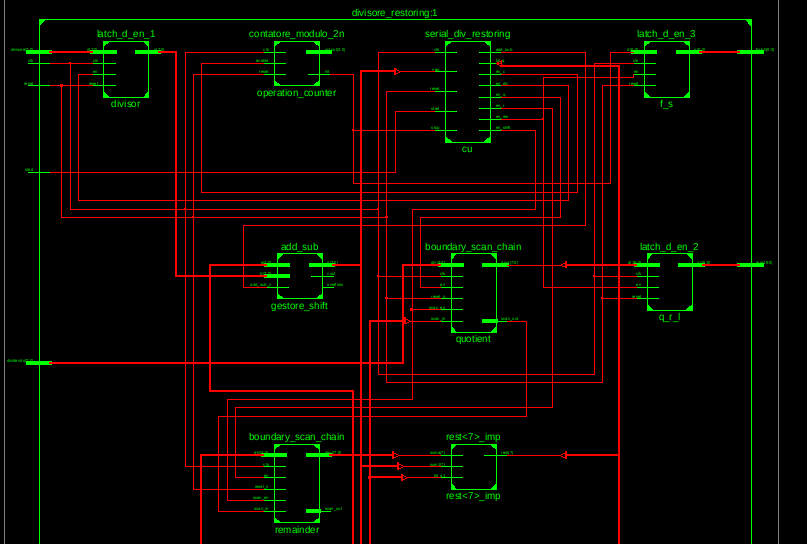
\includegraphics[scale=0.6]{esercizio14/images/div_restoring.png}
	\caption{Divisore restoring}
\end{figure}

Il circuito � molto simile a quello utilizzato per sviluppare un moltiplicatore
di Booth \ref{Booth}, cambia radicalmente per� in che modo i bit
vengono trattati difatti la macchina a stati finiti consiste di sei
stati: 
\begin{itemize}
\item idle stato di riposo, attende il segnale di avvio di una computazione;
\item init, in cui avviene l' inizializzazione delle scan chain, in questo
caso q ed r (q caricato con il valore del dividendo ed r inzializzato
a 0) e un registro per salvare il valore del divisore;
\item shift in cui i dati ( q ed r ) vengono shiftati a sinistra ( in Booth
i dati shiftano a destra);
\item sub in cui viene effettuata la sottrazione, nel caso il risultato
sia un numero negativo si ritorna in shift altrimenti, si procede
nello stato set\_1 che setta ad uno il bit da dover shiftare all'
interno di q, tale shift avverr� nello stato shift1. 
\end{itemize}
Il segnale di terminazione della computazione viene attivato quando
il contatore segnala un numero di operazioni pari al numero di bit
del dividendo.

\subsection{Codice}

\href{run:progetti/div_rest/div_rest.xise}{Divisore Restoring ISE}\selectlanguage{italian}%

